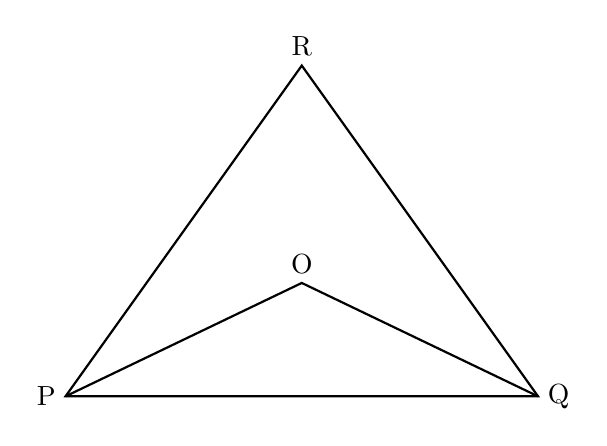
\begin{tikzpicture}[scale=1.2]

    % --- Define Coordinates ---
    % Vertex P at the bottom-left
    \coordinate (P) at (0,0);
    
    % Vertex Q at the bottom-right
    % Setting the base width to be visually proportional
    \coordinate (Q) at (5,0);
    
    % Vertex R at the top
    % Centered horizontally between P and Q, height chosen to match proportions
    \coordinate (R) at (2.5, 3.5);
    
    % Internal vertex O
    % Centered horizontally, positioned lower in the triangle
    \coordinate (O) at (2.5, 1.2);

    % --- Draw Lines ---
    % Draw the outer triangle PQR
    \draw[thick] (P) -- (Q) -- (R) -- cycle;

    % Draw the internal segments connecting P and Q to O
    \draw[thick] (P) -- (O) -- (Q);

    % --- Place Labels ---
    % Label P to the left of the vertex
    \node[left] at (P) {P};
    
    % Label Q to the right of the vertex
    \node[right] at (Q) {Q};
    
    % Label R above the top vertex
    \node[above] at (R) {R};
    
    % Label O above the internal vertex point
    \node[above] at (O) {O};

\end{tikzpicture}